% RESULTADOS PARA ANISOTROPÍAS EN RA PARA LOS ICRC
  \section{Anisotropías en ascensión recta en los archivos del ICRC 2017 y ICRC 2019}

% ---> 8 EeV 
    \subsection{Eventos por encima de 8 EeV }

% ------> CARACTERISTICAS
     % \subsubsection{Características de los datos analizados}

% ------> ICRC 2017
      \subsubsection{Resultados para los datos del ICRC 2017}

      Para este apartado analicé el archivo de datos de la tesis de doctorado de Oscar Taborda, solamente los eventos 6T5. El rango de tiempo en el cual hice  el análisis es entre 1072969615 y 1472688000 ( 2004-01-01 15:06:55 y 2016-11-01 0:00:00 )

      Sabemos que para energía mayores de 8 EeV, aparece el dipolo en sidérea.

      En las Fig.\,\ref{fig:8EeV_sin_peso_ICRC2017_raw} y \ref{fig:8EeV_sin_peso_ICRC2017_cor} se muestra la amplitud del primer armónico sin considerar el peso de los hexágonos. Está figura es compatible con la Fig. 5.7.b, página 90 de la tesis de Taborda.

        \begin{figure}[H]
        
          \begin{subfigure}[b]{\textwidth}
          \centering
            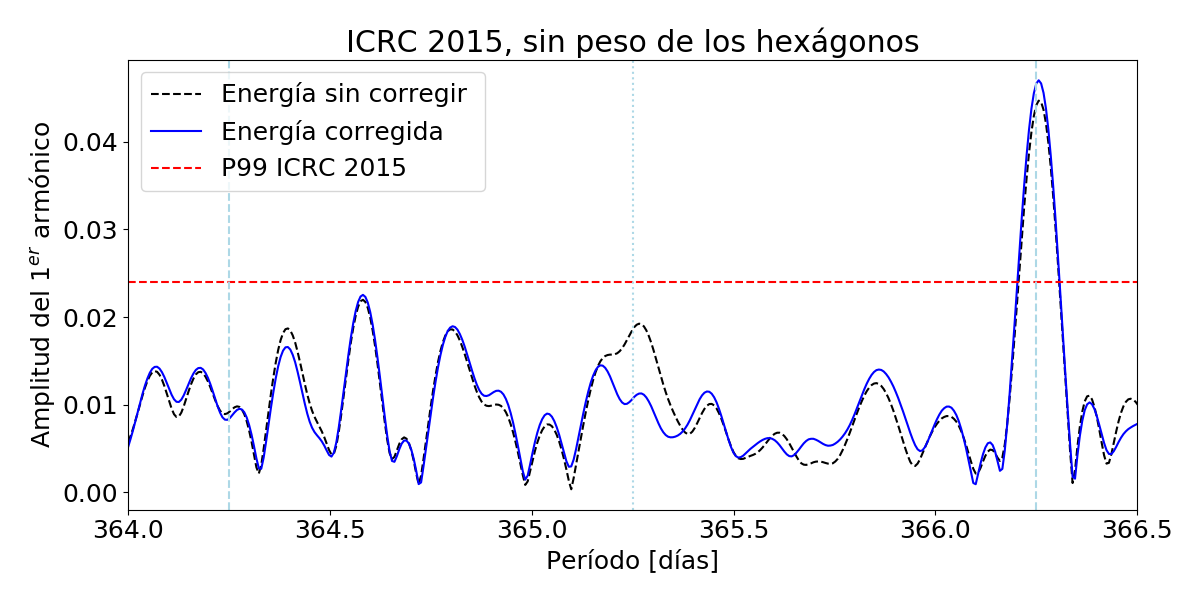
\includegraphics[width=\textwidth]{../0_Introduccion/ICRC/ICRC2017_Ecor_Eraw.png}
            \caption{Sin peso de la cantidad de tanques activos. }  \label{fig:8EeV_sin_peso_ICRC2017_raw}
          \end{subfigure}%
        
          \begin{subfigure}[b]{\textwidth}
          \centering
            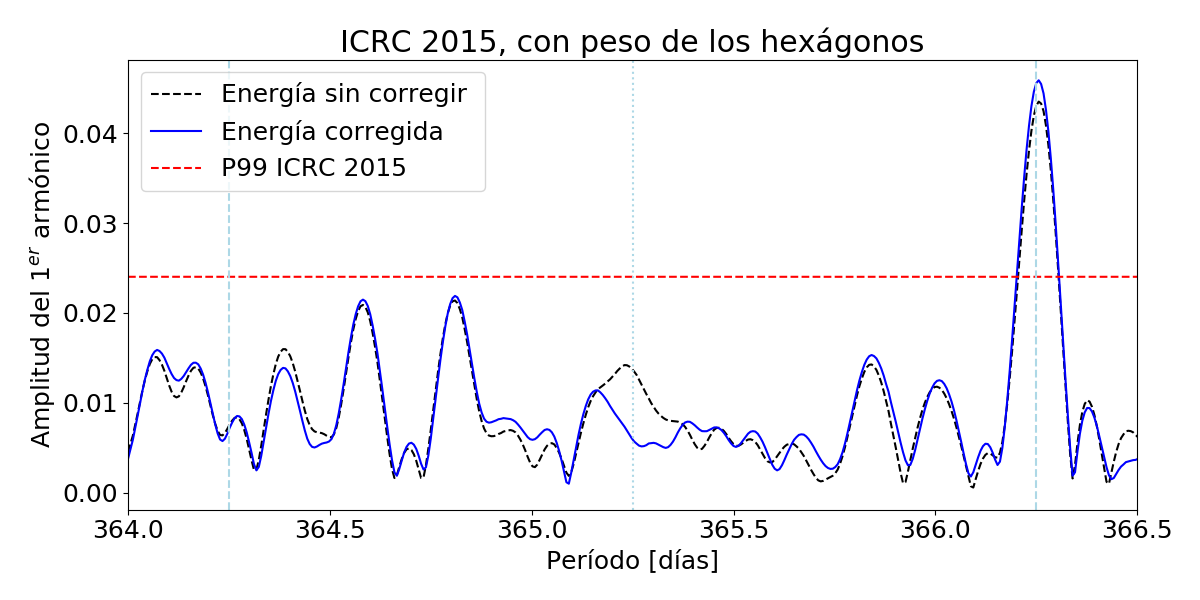
\includegraphics[width=\textwidth]{../0_Introduccion/ICRC/ICRC2017_Ecor_Eraw_hex.png}
            \caption{Con peso de la cantidad de tanques activos. }  \label{fig:8EeV_sin_peso_ICRC2017_cor}
          \end{subfigure}
          \caption{Primer armónico en ascensión recta de los datos del ICRC 2017}
        \end{figure}

      Con esto podemos decir que el código para la anisotropía funciona para el caso donde no se considera los hexágonos. No tengo un referencia para comparar las anisotropías con el peso de los hexágonos, solamente el valor del pico del dipolo.

% ------> ICRC 2019
      \subsubsection{Resultados para los datos del ICRC 2019}
      
      Este es el conjunto de archivos donde se hicieron modificaciones como el uso de una nueva reconstrucción y la corrección del clima. Usé solamente los eventos 6T5. El rango de tiempo en el cual hice  el análisis es entre 1072969615 y 1535789456 ( 2004-01-01 15:06:55 y   2018-09-01 08:10:56)

      \begin{figure}[H]
        \centering
        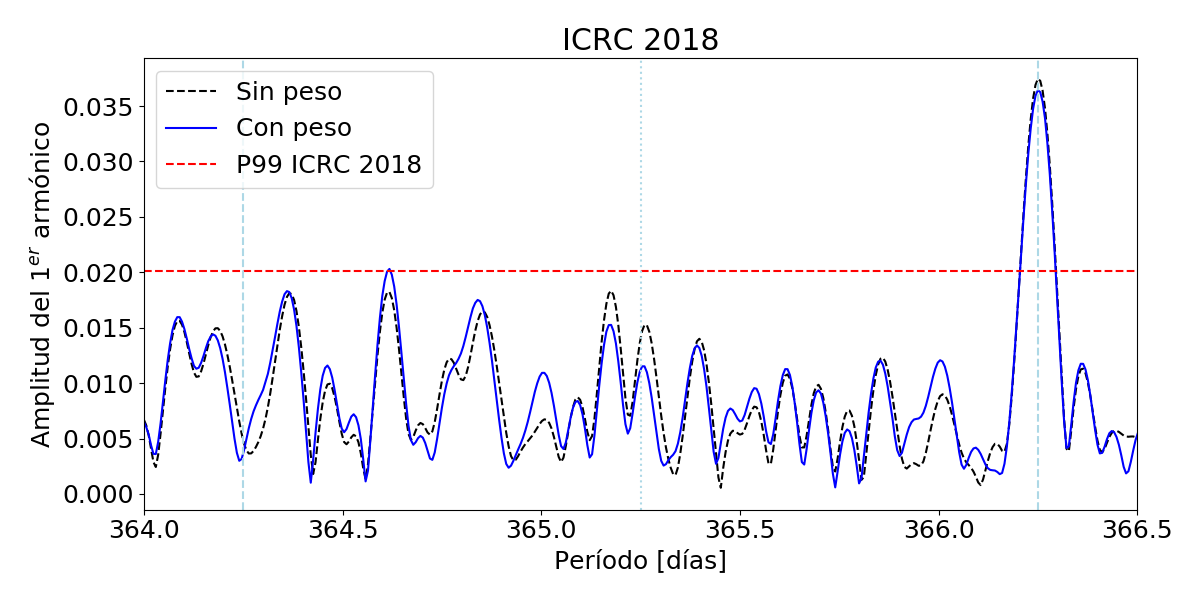
\includegraphics[width=\textwidth]{../0_Introduccion/ICRC/ICRC2019_Eraw_Eraw_hex.png}
        \caption{Primer armónico en ascensión recta de los datos del ICRC 2019.} \label{fig:8EeV_con_peso_ICRC2019}
      \end{figure}


      
